Per poter assicurare una conduzione e uno sviluppo del progetto che soddisfino le scadenze, il gruppo ha deciso di ripartire il lasso di tempo che va dalla sua formazione fino alla revisione di accettazione nelle seguenti fasi: 

\begin{itemize} 
	\item analisi dei requisiti; 
	\item consolidamento dei requisiti; 
	\item progettazione della \glock{technology baseline};
	\item progettazione e codifica del \glock{proof of concept} e funzionalità essenziali (incrementi 1-3);
	\item progettazione dell'architettura ed ulteriore implementazione di funzionalità (incrementi 4-6);
	\item completamento dell'implementazione e raffinamento delle funzionalità (incrementi 7-9);
	\item validazione e collaudo.
\end{itemize}
Ogni fase verrà poi frammentata in sotto periodi, ognuno dei quali individua più attività, le quali, possono essere svolte sia sequenzialmente, sia con un certo grado di parallelismo in base alle dipendenze che sussistono tra di loro. 

% ============================================

\subsection{Analisi dei requisiti} 
L’attività di analisi dei requisiti ha inizio il giorno 31-10-2021, successivamente alla formazione dei gruppi, suddivisa in cinque periodi, con termine fissato per il giorno 11-01-2021, giorno di consegna dei documenti in ingresso alla revisione dei requisiti. 

\subsubsection{Ruoli attivi} 
Durante questa attività è necessaria la presenza dei seguenti ruoli: 
\begin{itemize} 
	\item responsabile; 
	\item amministratore; 
	\item analista; 
	\item verificatore. 
\end{itemize} 

\subsubsection{Periodi} 
L'attività di analisi dei requisiti è stata suddivisa nei seguenti cinque periodi: 

\paragraph{Primo periodo: dal 31-10-2021 al 05-12-2021} 
\begin{itemize} 
	\item \textbf{Analisi dei capitolati}: studio individuale dei \glock{capitolati} e discussione interna al gruppo dei pregi e svantaggi individuati da ogni componente, in modo da indirizzare l’interesse del gruppo su certi \glock{capitolati} piuttosto che su altri; 
	\item \textbf{ricerca}: individuazione e studio degli strumenti e delle tecnologie di supporto da utilizzare per la gestione del progetto; 
	\item \textbf{studio di fattibilità}: impostato sulla base dell'analisi dei \glock{capitolati} fatta in precedenza; 
	\item \textbf{pianificazione attività}: decisione dell'organizzazione interna al gruppo riguardo i ruoli da assegnare ed i compiti da svolgere. 
\end{itemize} 

\paragraph{Secondo periodo: dal 05-12-2021 al 17-12-2021} 
\begin{itemize} 
	\item \textbf{Scelta del capitolato}: decisione definitiva riguardo il \glock{capitolato} scelto; 
	\item \textbf{normazione}: scelta delle regole da adottare durante lo sviluppo del progetto riguardanti i 
	processi primari e processi organizzativi; 
	\item \textbf{studio di fattibilità}: fine dello \dext{Studio di fattibilità v1.0.0}, basato sul \glock{capitolato} scelto. 
\end{itemize} 

\paragraph{Terzo periodo: dal 18-12-2021 al 29-12-2021} 
\begin{itemize} 
	\item \textbf{Analisi dei casi d'uso}: analisi del prodotto e dei casi d’uso; 
	\item \textbf{norme di progetto}: stesura delle \dext{Norme di progetto v1.0.0}; 
	\item \textbf{piano di progetto}: stesura del \dext{Piano di progetto v1.0.0}; 
	\item \textbf{analisi dei rischi}: individuazione dei rischi che possono presentarsi nello svolgimento del progetto. 
\end{itemize} 

\paragraph{Quarto periodo: dal 30-12-2021 al 07-01-2021} 
\begin{itemize} 
	\item \textbf{Analisi dei requisiti}: stesura dell’\dext{Analisi dei requisiti v1.0.0}; 
	\item \textbf{piano di qualifica}: stesura del \dext{Piano di qualifica v1.0.0}; 
	\item \textbf{glossario}: stesura del \dext{Glossario v1.0.0}. 
\end{itemize} 

\paragraph{Quinto periodo: dal 08-01-2021 al 11-01-2021} 
\begin{itemize} 
	\item \textbf{Revisione}: controllo della qualità di tutti i documenti redatti nella fase attuale; 
	\item \textbf{presentazione RR}: presentazione della documentazione alla revisione dei requisiti. 
\end{itemize} 


\newpage 

\begin{landscape} 
	\begin{figure}[h!] 
		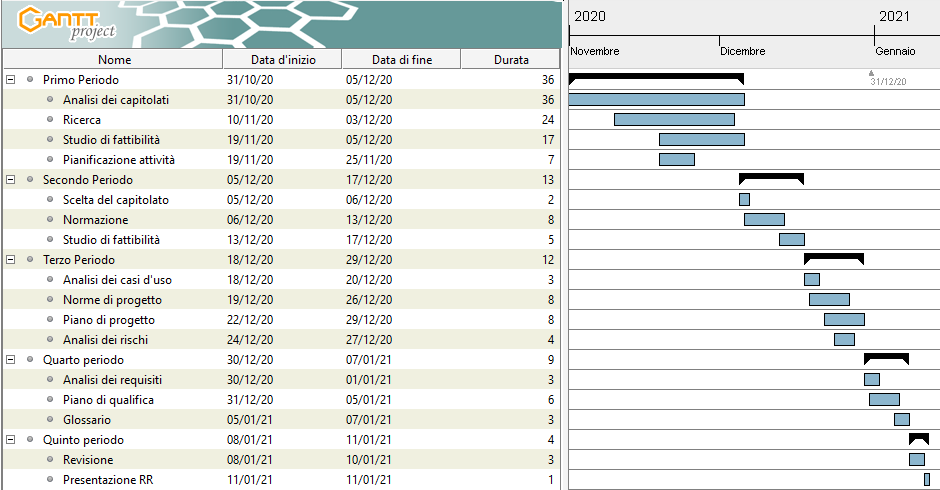
\includegraphics[width=24cm]{images/1_Analisi_dei_requisiti.png} 
		\caption{Pianificazione - Analisi dei requisiti} 
	\end{figure} 
\end{landscape} 

\newpage % ============================================

\subsection{Consolidamento dei Requisiti} 
L'attività di consolidamento dei requisiti ha inizio il giorno 12-01-2021, successivamente alla consegna del materiale in ingresso alla revisione dei requisiti, suddivisa in due periodi, con termine fissato 
per il giorno 17-01-2021 che precede la revisione dei requisiti del 18-01-2021. 

\subsubsection{Ruoli attivi} 
Durante questa attività è necessaria la presenza dei seguenti ruoli: 
\begin{itemize} 
	\item responsabile; 
	\item amministratore; 
	\item analista. 
\end{itemize} 

\subsubsection{Periodi} 
L'attività di consolidamento dei requisiti è stata suddivisa nei seguenti due periodi: 

\paragraph{Primo periodo: dal 12-01-2021 al 15-01-2021} 
\begin{itemize} 
	
	\item \textbf{Preparazione presentazione}: redazione della presentazione da portare in sede di revisione e studio individuale. 
	
\end{itemize}	 

\paragraph{Secondo periodo: dal 16-01-2021 al 17-01-2021} 
\begin{itemize} 
	
	\item \textbf{Analisi dei requisiti}: revisione ed eventuale aggiornamento dei requisiti. 
	
\end{itemize} 

\newpage 

\begin{landscape} 
	\begin{figure}[h!] 
		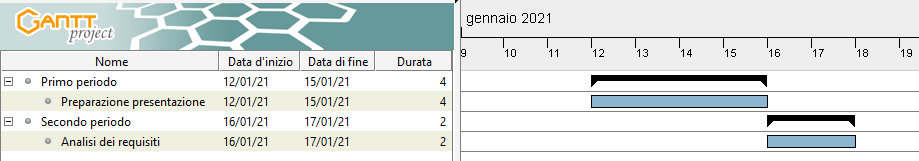
\includegraphics[width=24cm]{images/2_Consolidamento_dei_requisiti.png} 
		\caption{Pianificazione - Consolidamento dei requisiti} 
	\end{figure} 
\end{landscape} 

\newpage % ============================================

\subsection{Progettazione della \glock{technology baseline}} 
L'attività di progettazione della \glock{technology baseline} ha inizio il giorno 19-01-2021, successivamente alla revisione dei requisiti, suddivisa in tre periodi, con termine fissato per il giorno 07-03-2021 che precede la revisione di progettazione del 08-03-2021. 

\subsubsection{Ruoli attivi} 
Durante questa attività è necessaria la presenza dei seguenti ruoli: 
\begin{itemize} 
	\item responsabile; 
	\item amministratore; 
	\item analista; 
	\item progettista; 
	\item programmatore; 
	\item verificatore.
\end{itemize} 

\subsubsection{Periodi} 
L'attività di progettazione della \glock{technology baseline} è stata suddivisa nei seguenti periodi: 

\paragraph{Primo periodo: dal 19-01-2021 al 11-02-2021} 
\begin{itemize} 
	\item \textbf{Normazione}: revisione ed eventuale aggiornamento delle norme; 
	\item \textbf{aggiornamento della pianificazione}; 
	\item \textbf{aggiornamento della qualità}; 
	\item \textbf{analisi dei requisiti}: revisione ed eventuale aggiornamento dei casi d’uso e dei requisiti, in base alle indicazioni ricevute; 
	\item \textbf{ricerca}: studio degli strumenti e le tecnologie da utilizzare per lo sviluppo del 
	progetto; 
	\item \textbf{verifica}: controllo della qualità di tutti i prodotti sviluppati durante il periodo attuale. 
\end{itemize} 

\paragraph{Secondo periodo: dal 12-02-2021 al 03-03-2021} 
\begin{itemize} 
	\item \textbf{Normazione}: aggiornamento delle norme; 
	\item \textbf{progettazione}: progettazione dell'architettura del sistema e di un primo \glock{proof of concept};
	\item \textbf{aggiornamento della pianificazione}; 
	\item \textbf{codifica}: prima implementazione del \glock{proof of concept} progettato; 
	\item \textbf{stesura della lettera di presentazione}: scrittura della lettera di presentazione con la quale ci si candida alla revisione di progettazione; 
	\item \textbf{verifica}: controllo della qualità di tutti i prodotti sviluppati durante il periodo attuale. 
\end{itemize}	 

\paragraph{Terzo periodo: dal 04-03-2021 al 07-03-2021} 
\begin{itemize} 
	\item \textbf{Preparazione presentazione}: redazione della presentazione da portare in sede di revisione e studio individuale. 
\end{itemize} 

\newpage 

\begin{landscape} 
	\begin{figure}[h!] 
		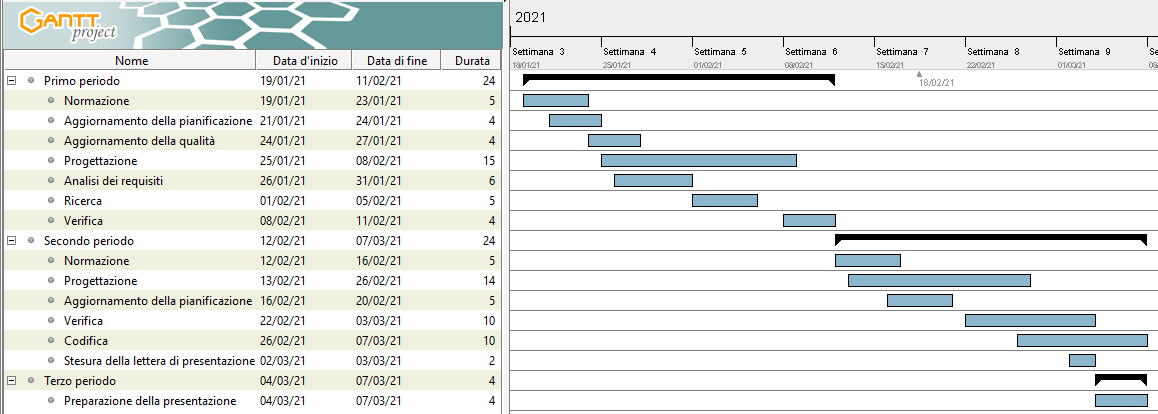
\includegraphics[width=24cm]{images/3_Progettazione_della_Technology.png} 
		\caption{Pianificazione - Progettazione della Technology Baseline} 
	\end{figure} 
\end{landscape} 

\newpage % ============================================	

\subsection{Progettazione e codifica del proof of concept e funzionalità essenziali}
In questa prima fase di sviluppo verranno implementate le funzionalità base dell'architettura, che non comprenderà quindi tutte le componenti richieste dal capitolato, ma solo quelle essenziali.
\newline
Nei prossimi tre incrementi, quindi, verranno sviluppate le componenti e le funzionalità base dell'applicazione. \newline
Di seguito viene riportato il dettaglio di ogni incremento.

\subsubsection{Incremento 1}
L'incremento 1 prevede la progettazione e codifica delle componenti software per la realizzazione del \glock{proof of concept}. Si prevede di svolgere quanto segue:
\begin{itemize}
	\item configurazione di \glock{Angular JS}.
	\item configurazione di \glock{Docker}.
\end{itemize}

\paragraph{Ruoli attivi}
Durante questa fase è necessaria la presenza dei seguenti ruoli: 
\begin{itemize} 
	\item responsabile; 
	\item amministratore; 
	\item progettista; 
	\item programmatore; 
	\item verificatore.
\end{itemize}

\paragraph{Periodi e attività}
\subparagraph{Unico periodo: dal 09-03-2021 al 18-03-2021}

\begin{itemize}
	\item \textbf{analisi delle tecnologie:} analisi del funzionamento di \glock{Angular JS} e \glock{Docker};
	\item \textbf{progettazione:} progettazione della configurazione per \glock{Angular JS} ed integrazione con \glock{Docker};
	\item \textbf{codifica:} implementazione della configurazione;
	\item \textbf{verifica:} controllo sul funzionamento della configurazione.
\end{itemize} 			

 % ============================================

\subsubsection{Incremento 2}
L'incremento 2 prevede la progettazione di dettaglio e codifica delle componenti software per andare a costituire un \glock{proof of concept}. Si prevede di svolgere quanto segue:
\begin{itemize}
	\item ;
	\item ;
	\item .
\end{itemize}

\paragraph{Ruoli attivi}
Durante questa fase è necessaria la presenza dei seguenti ruoli: 
\begin{itemize} 
	\item responsabile; 
	\item amministratore; 
	\item progettista; 
	\item programmatore; 
	\item verificatore.
\end{itemize}

\paragraph{Periodi e attività}
\subparagraph{Unico periodo: dal 19-03-2021 al 30-03-2021}
\begin{itemize}
	\item ;
	\item ;
	\item ;
	\item ;
	\item .
\end{itemize}

 % ============================================

\subsubsection{Incremento 3}
L'incremento 3 prevede la progettazione di dettaglio e codifica delle componenti software per andare a costituire un \glock{proof of concept}. Si prevede di svolgere quanto segue:
\begin{itemize}
	\item ;
	\item ;
	\item .
\end{itemize}
Con la fine di questo incremento, si va a costituire un primo \glock{proof of concept} del prodotto che potrà essere mostrato al committente e al proponente.

\paragraph{Ruoli attivi}
Durante questa fase è necessaria la presenza dei seguenti ruoli: 
\begin{itemize} 
	\item responsabile; 
	\item amministratore; 
	\item progettista; 
	\item programmatore; 
	\item verificatore.
\end{itemize}

\paragraph{Periodi e attività}
\subparagraph{Unico periodo: dal 31-03-2021 al 08-04-2021}
\begin{itemize}
	\item ;
	\item ;
	\item ;
	\item ;
	\item .
\end{itemize}
 
\newpage 

\begin{landscape} 
	\begin{figure}[h!] 
		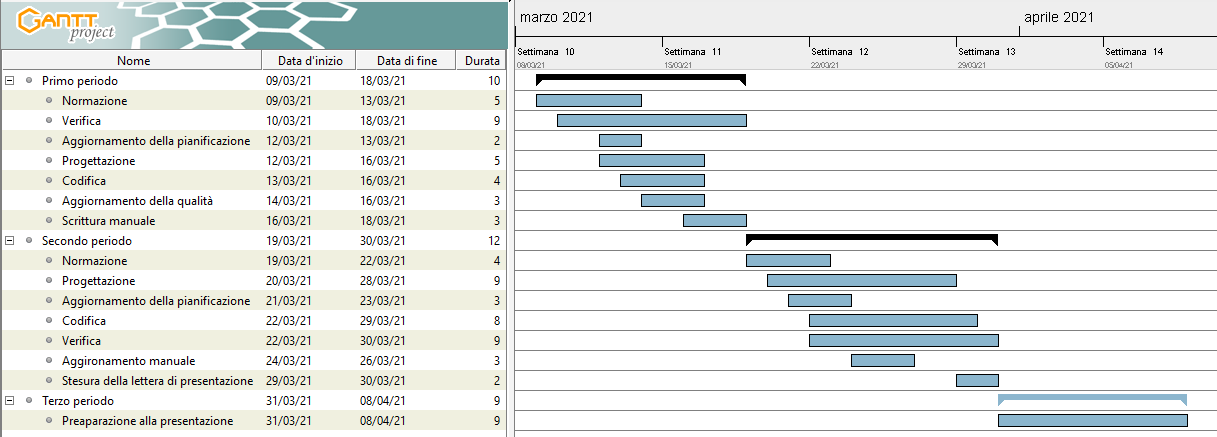
\includegraphics[width=24cm]{images/4_Progettazione_e_codifica.png} 
		\caption{Pianificazione - Progettazione e codifica} 
	\end{figure} 
\end{landscape} 

\newpage 

 % ============================================
 
 